\chapter{Introduction}\label{sec:intro}
\begin{flushright}{\slshape    
The most important contribution of management in the 20th century\\
was to increase manual worker productivity fifty-fold.\\
The most important contribution of management in the 21st century\\
will be to increase knowledge worker productivity\\
— hopefully by the same percentage} \\ \medskip
--- Peter Drucker~\cite{drucker1999}
\end{flushright}

When Peter Drucker became aware that the automation of manual labour was progressing faster than that of knowledge work, he said these words at the end of the $20^{th}$ century in 1999. Between both types of work lies a pronounced difference: The course of manual work is determined by physical laws, is often very structured and thus offers great potential for easy automation. Knowledge work requires one to "think for a living" and is thus shaped by the individuality of the knowledge worker. As each worker has a different knowledge background and uses information differently, this type of work is very flexible and often no task is ever executed exactly the same. This flexibility incurs making many decisions, as small as they may be - all need to be made by the knowledge worker based upon information.

Now, 20 years later, numerous knowledge repositories and assistance systems for knowledge workers exist, helping make decisions more informed and faster. From these systems, logs can be extracted, which document the course of a process instance from its beginning to its completion. Instances of a process are henceforth referred to as cases.\\

This thesis makes uses of these logs and presents a step towards a system that can actively assist the knowledge worker by predicting the activity which would usually be executed next in the context of a case's execution. One possible outlook is the further processing of this prediction by a process guidance system for knowledge workers, ultimately giving recommendations. A special type of neural networks was used to obtain the predictions. \autoref{fig:next-activity-prediction} illustrates the raw input data to the network: the sequence of elapsed activities and the attached data attributes.\\

\begin{figure}
    \centering
    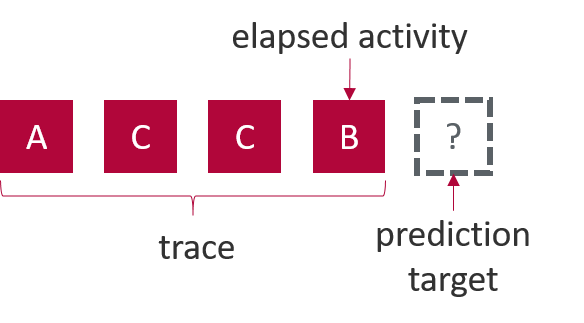
\includegraphics[width=\textwidth]{gfx/next-activity.png}
    \caption{Predicting the next activity, TODO replace}
    \label{fig:next-activity-prediction}
\end{figure}

The application of Predictive Analytics in Process Science is fairly new, and is now commonly referred to as Predictive Process Monitoring. A preliminary definition is delivered along with comprehensive information on the other areas in \autoref{chap:background}. As Predictve Process Monitoring is a new domain, only a small number of publications have addressed the prediction of the next activity. Much more work exists on older prediction problems, e.g. prediction of predicate conformance or completion time, to name two. These related works are presented in \autoref{chap:related-work}.

Furthermore, the fact that no domain-specific benchmarking dataset for this kind of problem exists yet, makes the few existing publications hard to compare, as they work on different data. There is however a tendency to make use of the datasets of the Business Process Intelligence Competition (BPIC)~\cite{BPIC2011, BPIC2012, BPIC2017}, which publishes a new dataset for every year.

Lastly, the next-activity prediction problem has not been related to similar problems in domains in which more work has already been done. Some of these are also presented in \autoref{chap:related-work}.\\

This thesis addresses these three shortcomings by proposing a revised prediction model that was inspired by predictive models applied in the area of Natural Language Processing (NLP) and stems from injecting engineered features on an intermediate network layer. The approach is tested on the datasets of BPIC 2011 and 2012 and compared to two implementations reverse-engineered from the following publications, thus allowing a direct comparison (see \autoref{chap:contribution}):

\begin{enumerate}
    \item \textit{A Deep Learning Approach for Predicting Process Behaviour at Runtime} by Evermann et al.~\cite{evermann2016} \item\textit{Deep Learning Process Prediction with Discrete and Continuous Data Features} by Schönig et al.~\cite{schoenig2018}.
\end{enumerate}

Over the course of reverse-engineering the comparison models and the subsequent evaluation, widely divergent understandings and approaches with regard to the structure of sequential data input for neural networks were uncovered. To contribute to a better understanding in this area, a comparison of the perceived possibilities was incorporated into the evaluation. These findings are presented along with implementation details and performance measures in \autoref{chap:evaluation}.

The thesis ends with \autoref{chap:conclusion}, which summarizes the findings and the accomplishments of this work that began in September 2018. Furthermore it gives pointers with which to improve and continue the work in this active field.